% 若编译失败,且生成 .synctex(busy) 辅助文件,可能有两个原因:
% 1. 需要插入的图片不存在:Ctrl + F 搜索 'figure' 将这些代码注释/删除掉即可
% 2. 路径/文件名含中文或空格:更改路径/文件名即可

% --------------------- 文章宏包及相关设置 --------------------- %
% >> ------------------ 文章宏包及相关设置 ------------------ << %
% 设定文章类型与编码格式
\documentclass[UTF8]{report}		

% 自定义宏定义
    \def\N{\mathbb{N}}
    \def\F{\mathbb{F}}
    \def\Z{\mathbb{Z}}
    \def\Q{\mathbb{Q}}
    \def\R{\mathbb{R}}
    \def\C{\mathbb{C}}
    \def\T{\mathbb{T}}
    \def\S{\mathbb{S}}
    \def\A{\mathbb{A}}
    \def\I{\mathscr{I}}
    \def\Im{\mathrm{Im\,}}
    \def\Re{\mathrm{Re\,}}
    \def\d{\mathrm{d}}
    \def\p{\partial}

% 导入基本宏包
    \usepackage[UTF8]{ctex}     % 设置文档为中文语言
    \usepackage[colorlinks, linkcolor=blue, anchorcolor=blue, citecolor=blue, urlcolor=blue]{hyperref}  % 宏包:自动生成超链接 (此宏包与标题中的数学环境冲突)
    % \usepackage{docmute}    % 宏包:子文件导入时自动去除导言区,用于主/子文件的写作方式,\include{./51单片机笔记}即可。注:启用此宏包会导致.tex文件capacity受限。
    \usepackage{amsmath}    % 宏包:数学公式
    \usepackage{mathrsfs}   % 宏包:提供更多数学符号
    \usepackage{amssymb}    % 宏包:提供更多数学符号
    \usepackage{pifont}     % 宏包:提供了特殊符号和字体
    \usepackage{extarrows}  % 宏包:更多箭头符号


% 文章页面margin设置
    \usepackage[a4paper]{geometry}
        \geometry{top=1in}
        \geometry{bottom=1in}
        \geometry{left=0.75in}
        \geometry{right=0.75in}   % 设置上下左右页边距
        \geometry{marginparwidth=1.75cm}    % 设置边注距离(注释、标记等)

% 配置数学环境
    \usepackage{amsthm} % 宏包:数学环境配置
    % theorem-line 环境自定义
        \newtheoremstyle{MyLineTheoremStyle}% <name>
            {11pt}% <space above>
            {11pt}% <space below>
            {}% <body font> 使用默认正文字体
            {}% <indent amount>
            {\bfseries}% <theorem head font> 设置标题项为加粗
            {:}% <punctuation after theorem head>
            {.5em}% <space after theorem head>
            {\textbf{#1}\thmnumber{#2}\ \ (\,\textbf{#3}\,)}% 设置标题内容顺序
        \theoremstyle{MyLineTheoremStyle} % 应用自定义的定理样式
        \newtheorem{LineTheorem}{Theorem.\,}
    % theorem-block 环境自定义
        \newtheoremstyle{MyBlockTheoremStyle}% <name>
            {11pt}% <space above>
            {11pt}% <space below>
            {}% <body font> 使用默认正文字体
            {}% <indent amount>
            {\bfseries}% <theorem head font> 设置标题项为加粗
            {:\\ \indent}% <punctuation after theorem head>
            {.5em}% <space after theorem head>
            {\textbf{#1}\thmnumber{#2}\ \ (\,\textbf{#3}\,)}% 设置标题内容顺序
        \theoremstyle{MyBlockTheoremStyle} % 应用自定义的定理样式
        \newtheorem{BlockTheorem}[LineTheorem]{Theorem.\,} % 使用 LineTheorem 的计数器
    % definition 环境自定义
        \newtheoremstyle{MySubsubsectionStyle}% <name>
            {11pt}% <space above>
            {11pt}% <space below>
            {}% <body font> 使用默认正文字体
            {}% <indent amount>
            {\bfseries}% <theorem head font> 设置标题项为加粗
            {:\\ \indent}% <punctuation after theorem head>
            {0pt}% <space after theorem head>
            {\textbf{#3}}% 设置标题内容顺序
        \theoremstyle{MySubsubsectionStyle} % 应用自定义的定理样式
        \newtheorem{definition}{}

%宏包:有色文本框(proof环境)及其设置
    \usepackage[dvipsnames,svgnames]{xcolor}    %设置插入的文本框颜色
    \usepackage[strict]{changepage}     % 提供一个 adjustwidth 环境
    \usepackage{framed}     % 实现方框效果
        \definecolor{graybox_color}{rgb}{0.95,0.95,0.96} % 文本框颜色。修改此行中的 rgb 数值即可改变方框纹颜色,具体颜色的rgb数值可以在网站https://colordrop.io/ 中获得。(截止目前的尝试还没有成功过,感觉单位不一样)(找到喜欢的颜色,点击下方的小眼睛,找到rgb值,复制修改即可)
        \newenvironment{graybox}{%
        \def\FrameCommand{%
        \hspace{1pt}%
        {\color{gray}\small \vrule width 2pt}%
        {\color{graybox_color}\vrule width 4pt}%
        \colorbox{graybox_color}%
        }%
        \MakeFramed{\advance\hsize-\width\FrameRestore}%
        \noindent\hspace{-4.55pt}% disable indenting first paragraph
        \begin{adjustwidth}{}{7pt}%
        \vspace{2pt}\vspace{2pt}%
        }
        {%
        \vspace{2pt}\end{adjustwidth}\endMakeFramed%
        }

% 外源代码插入设置
    % matlab 代码插入设置
    \usepackage{matlab-prettifier}
        \lstset{
            style=Matlab-editor,  % 继承matlab代码颜色等
        }
    \usepackage[most]{tcolorbox} % 引入tcolorbox包 
    \usepackage{listings} % 引入listings包
        \tcbuselibrary{listings, skins, breakable}
        \lstdefinestyle{matlabstyle}{
            language=Matlab,
            basicstyle=\small,
            breakatwhitespace=false,
            breaklines=true,
            captionpos=b,
            keepspaces=true,
            numbers=left,
            numbersep=15pt,
            showspaces=false,
            showstringspaces=false,
            showtabs=false,
            tabsize=2
        }
        \newtcblisting{matlablisting}{
            arc=0pt,
            top=0pt,
            bottom=0pt,
            left=1mm,
            listing only,
            listing style=matlabstyle,
            breakable,
            colback=white   % 选一个合适的颜色
        }

% table 支持
    \usepackage{booktabs}   % 宏包:三线表
    \usepackage{tabularray} % 宏包:表格排版
    \usepackage{longtable}  % 宏包:长表格

% figure 设置
    \usepackage{graphicx}  % 支持 jpg, png, eps, pdf 图片 
    \usepackage{svg}       % 支持 svg 图片
        \svgsetup{
            % 指向 inkscape.exe 的路径
            inkscapeexe = D:/aa_my_apps_main/Inkscape/bin/inkscape.exe, 
            % 一定程度上修复导入后图片文字溢出几何图形的问题
            inkscapelatex = false                 
        }

% 图表进阶设置
    \usepackage{caption}    % 图注、表注
        \captionsetup[figure]{name=图}  
        \captionsetup[table]{name=表}
        \captionsetup{labelfont=bf, font=small}
    \usepackage{float}     % 图表位置浮动设置 

% 圆圈序号自定义
    \newcommand*\circled[1]{\tikz[baseline=(char.base)]{\node[shape=circle,draw,inner sep=0.8pt, line width = 0.03em] (char) {\small \bfseries #1};}}   % TikZ solution

% 列表设置
\usepackage{enumitem}   % 宏包:列表环境设置
    \setlist[enumerate]{itemsep=0pt, parsep=0pt, topsep=0pt, partopsep=0pt, leftmargin=3.5em} 
    \setlist[itemize]{itemsep=0pt, parsep=0pt, topsep=0pt, partopsep=0pt, leftmargin=3.5em}
    \newlist{circledenum}{enumerate}{1} % 创建一个新的枚举环境  
    \setlist[circledenum,1]{  
        label=\protect\circled{\arabic*}, % 使用 \arabic* 来获取当前枚举计数器的值,并用 \circled 包装它  
        ref=\arabic*, % 如果需要引用列表项,这将决定引用格式(这里仍然使用数字)
        itemsep=0pt, parsep=0pt, topsep=0pt, partopsep=0pt, leftmargin=3.5em
    }  
    

% 文章默认字体设置
\usepackage{fontspec}   % 宏包:字体设置
    \setmainfont{SimSun}    % 设置中文字体为宋体字体
    \setmainfont{Times New Roman} % 设置英文字体为Times New Roman

% 文章序言设置
    \newcommand{\cnabstractname}{序言}
    \newenvironment{cnabstract}{%
        \par\Large
        \noindent\mbox{}\hfill{\bfseries \cnabstractname}\hfill\mbox{}\par
        \vskip 2.5ex
        }{\par\vskip 2.5ex}

% 参考文献引用设置
    \bibliographystyle{unsrt}   % 设置参考文献引用格式为unsrt
    \newcommand{\upcite}[1]{\textsuperscript{\cite{#1}}}     % 自定义上角标式引用

% 各级标题自定义设置
    \usepackage{titlesec}   
    % chapter
        \titleformat{\chapter}[hang]{\normalfont\Large\bfseries\centering}{Homework \thechapter :}{10pt}{}
        \titlespacing*{\chapter}{0pt}{-30pt}{10pt} % 控制上方空白的大小
    % section
        \titleformat{\section}[hang]{\normalfont\large\bfseries}{\thesection}{8pt}{}
    % subsection
        %\titleformat{\subsubsection}[hang]{\normalfont\bfseries}{}{8pt}{}
    % subsubsection
        %\titleformat{\subsubsection}[hang]{\normalfont\bfseries}{}{8pt}{}

% --------------------- 文章宏包及相关设置 --------------------- %
% >> ------------------ 文章宏包及相关设置 ------------------ << %



% ------------------------ 文章信息区 ------------------------ %
% >> --------------------- 文章信息区 --------------------- << %
% 页眉页脚设置

\usepackage{fancyhdr}   %宏包:页眉页脚设置
    \pagestyle{fancy}
    \fancyhf{}
    \cfoot{\thepage}
    \renewcommand\headrulewidth{1pt}
    \renewcommand\footrulewidth{0pt}
    \chead{光学作业,\ 丁毅,\ 2023K8009908031}
    \lhead{Homework \thechapter}
    \rhead{dingyi233@mails.ucas.ac.cn}

%文档信息设置
\title{光学作业\\ Homework of Optics}
\author{丁毅\\ \footnotesize 中国科学院大学,北京 100049\\ Yi Ding \\ \footnotesize University of Chinese Academy of Sciences, Beijing 100049, China}
\date{\footnotesize 2024.9 -- 2025.1}
% >> --------------------- 文章信息区 --------------------- << %
% ------------------------ 文章信息区 ------------------------ %

% 开始编辑文章

\begin{document}
\zihao{5}           % 设置全文字号大小

% ------------------------ 封面序言与目录 ------------------------ %
% >> --------------------- 封面序言与目录 --------------------- << %
% 封面
    \maketitle\newpage  
    \pagenumbering{Roman} % 页码为大写罗马数字
    \thispagestyle{fancy}   % 显示页码、页眉等

% 序言
    \begin{cnabstract}\normalsize 
        本文为笔者本科时的“光学”课程作业(Homework of Optics, 2024.9-2025.1)。由于个人学识浅陋,认识有限,文中难免有不妥甚至错误之处,望读者不吝指正,在此感谢。\par 
        我的邮箱是 dingyi233@mails.ucas.ac.cn。
    \end{cnabstract}
    \addcontentsline{toc}{chapter}{序言} % 手动添加为目录

% 不换页目录
    \setcounter{tocdepth}{0}
    \noindent\rule{\textwidth}{0.1em}   % 分割线
    \noindent\begin{minipage}{\textwidth}\centering 
        \vspace{1cm}
        \tableofcontents\thispagestyle{fancy}   % 显示页码、页眉等   
    \end{minipage}  
    \addcontentsline{toc}{chapter}{目录} % 手动添加为目录

% 收尾工作
    \newpage    
    \pagenumbering{arabic} 

% >> --------------------- 封面序言与目录 --------------------- << %
% ------------------------ 封面序言与目录 ------------------------ %

\chapter{2024.9.2 - 2024.9.8}\thispagestyle{fancy}

\section{求入射到光纤的角度满足的条件}

\begin{equation}
    n_0 \sin i = n_g \sin i', \quad n_g \sin (\frac{\pi}{2} - i') = n_c \sin \frac{\pi}{2} 
     \Longrightarrow i \leqslant \arcsin 
\end{equation}
    

\begin{figure}[H]\centering
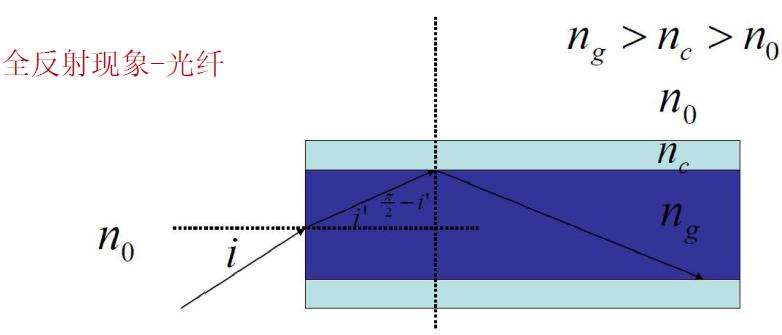
\includegraphics[width=0.55\textwidth]{assets/c6c9e6ef2f6755ead534508010ad0452 (2).jpg}
\caption{\textbf{求入射到光纤的角度满足的条件}}\label{求入射到光纤的角度满足的条件}
\end{figure}

\section{推导光线轨迹方程}

在 $x$-$y$ 平面中,设 $y = y(x)$ 表示光线的轨迹方程,$n = n(y)$ 表示介质的折射率。由几何关系,我们有:
\begin{equation}
\frac{\mathrm{d} y }{\mathrm{d} x } = \tan \theta = \frac{1}{\tan i} = \frac{\sqrt{1-\sin^2 i}}{\sin i} 
\end{equation}

由折射定律,记 $[n(y)\sin i(y)]_{y=0} = C$ ,则我们有:
\begin{equation}
n(y)\sin i(y) = C \Longrightarrow \frac{\mathrm{d} y }{\mathrm{d} x } = \frac{\sqrt{n^2 - C^2}}{C^2}, \quad \left(\frac{\mathrm{d} y }{\mathrm{d} x }\right)^{2} = \frac{n^2}{C^2} - 1
\end{equation}
两边同时对 $x$ 求导,得到:
\begin{equation}
2 \left(\frac{\mathrm{d} y }{\mathrm{d} x }\right) \left(\frac{\mathrm{d}^2 y }{\mathrm{d} x^2 }\right) = \frac{1}{C^2} \left(\frac{\mathrm{d} n^2 }{\mathrm{d} y }\right) \left(\frac{\mathrm{d} y }{\mathrm{d} x }\right) \Longrightarrow \frac{\mathrm{d}^2 y }{\mathrm{d} x^2 } = \frac{1}{2C^2}\cdot \frac{\mathrm{d} n^2 }{\mathrm{d} y } 
\end{equation}
也即
\begin{equation}
    \frac{\mathrm{d}^2 y }{\mathrm{d} x^2 } = \frac{1}{2n_0^2\sin^2 i}\cdot \frac{\mathrm{d} n^2 }{\mathrm{d} y } = \frac{1}{2n_0^2\cos^2 \theta}\cdot \frac{\mathrm{d} n^2 }{\mathrm{d} y } \quad 
\end{equation}
证毕。$\quad \square$

\begin{figure}[H]\centering
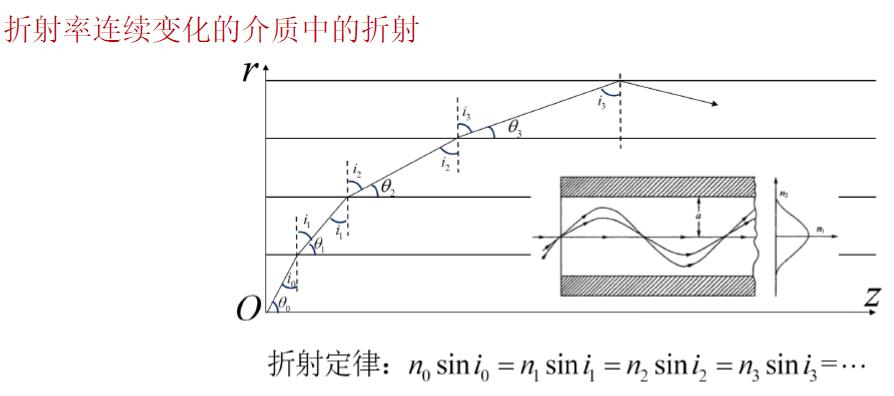
\includegraphics[width=0.8\textwidth]{assets/88b3f41951f9d3be9e2964935ebaf0f7.jpg}
\caption{\textbf{推导光线轨迹方程}}\label{推导光线轨迹方程}
\end{figure}

事实上,在三维坐标系中考虑上述过程,或者利用费马原理和变分法,又或考虑哈密顿光学,可以得到更一般的形式,称为光路方程:
\begin{equation}
    \nabla n=\frac{\mathrm{d}}{\mathrm{d}s}\left(n\frac{\mathrm{d}\vec{r}}{\mathrm{d}s}\,\right)
\end{equation}





















































































































\chapter{2024.9.2 - 2024.9.8}\thispagestyle{fancy}
\chapter{2024.9.9 - 2024.9.15}\thispagestyle{fancy}
\chapter{2024.9.16 - 2024.9.22}\thispagestyle{fancy}
\chapter{2024.9.23 - 2024.9.29}\thispagestyle{fancy}
\chapter{2024.9.30 - 2024.10.7}\thispagestyle{fancy}



\newpage
\href{https://www.latex-tables.com/}{Latex Table Editor} 示例:


\begin{longtblr}[caption={\bfseries 示例表格},label=tab:example]{
    hline{1,51} = {-}{0.08em},
    hline{2} = {-}{},
  }
   $x$& hello & $123.456$ \\
   $x$& hello & $123.456$ \\
   $x$& hello & $123.456$ \\
   $x$& hello & $123.456$ \\
   $x$& hello & $123.456$ \\
   $x$& hello & $123.456$ \\
   $x$& hello & $123.456$ \\
   $x$& hello & $123.456$ \\
   $x$& hello & $123.456$ \\
   $x$& hello & $123.456$ \\
   $x$& hello & $123.456$ \\
   $x$& hello & $123.456$ \\
   $x$& hello & $123.456$ \\
   $x$& hello & $123.456$ \\
   $x$& hello & $123.456$ \\
   $x$& hello & $123.456$ \\
   $x$& hello & $123.456$ \\
   $x$& hello & $123.456$ \\
   $x$& hello & $123.456$ \\
   $x$& hello & $123.456$ \\
   $x$& hello & $123.456$ \\
   $x$& hello & $123.456$ \\
   $x$& hello & $123.456$ \\
   $x$& hello & $123.456$ \\
   $x$& hello & $123.456$ \\
   $x$& hello & $123.456$ \\
   $x$& hello & $123.456$ \\
   $x$& hello & $123.456$ \\
   $x$& hello & $123.456$ \\
   $x$& hello & $123.456$ \\
   $x$& hello & $123.456$ \\
   $x$& hello & $123.456$ \\
   $x$& hello & $123.456$ \\
   $x$& hello & $123.456$ \\
   $x$& hello & $123.456$ \\
   $x$& hello & $123.456$ \\
   $x$& hello & $123.456$ \\
   $x$& hello & $123.456$ \\
   $x$& hello & $123.456$ \\
   $x$& hello & $123.456$ \\
   $x$& hello & $123.456$ \\
   $x$& hello & $123.456$ \\
   $x$& hello & $123.456$ \\
   $x$& hello & $123.456$ \\
   $x$& hello & $123.456$ \\
   $x$& hello & $123.456$ \\
   $x$& hello & $123.456$ \\
   $x$& hello & $123.456$ \\
   $x$& hello & $123.456$ \\
   $x$& hello & $123.456$ 
\end{longtblr}

\href{https://www.tablesgenerator.com/latex_tables#}{Create Latex Tables Online} 示例:

% Please add the following required packages to your document preamble:
% \usepackage{booktabs}
% \usepackage{longtable}
% Note: It may be necessary to compile the document several times to get a multi-page table to line up properly
\begin{longtable}[c]{ccc}
    \caption{\bfseries Create Latex Tables Online 示例}
    \label{tab:my-table}\\
    \toprule
    表头& 表头 & 表头 \\* \midrule
    \endfirsthead
    %
    \multicolumn{3}{c}%
    {{\bfseries Table \thetable :\ continued from previous page}} \\
    \toprule
    表头& 表头 & 表头 \\* \midrule
    \endhead
    %
    \bottomrule
    \endfoot
    %
    \endlastfoot
    %
     $x$ & hello  & $123.456$ \\
     $x$ & hello  & $123.456$ \\
     $x$ & hello  & $123.456$ \\
     $x$ & hello  & $123.456$ \\
     $x$ & hello  & $123.456$ \\
     $x$ & hello  & $123.456$ \\
     $x$ & hello  & $123.456$ \\
     $x$ & hello  & $123.456$ \\
     $x$ & hello  & $123.456$ \\
     $x$ & hello  & $123.456$ \\
     $x$ & hello  & $123.456$ \\
     $x$ & hello  & $123.456$ \\
     $x$ & hello  & $123.456$ \\
     $x$ & hello  & $123.456$ \\
     $x$ & hello  & $123.456$ \\
     $x$ & hello  & $123.456$ \\
     $x$ & hello  & $123.456$ \\
     $x$ & hello  & $123.456$ \\
     $x$ & hello  & $123.456$ \\
     $x$ & hello  & $123.456$ \\
     $x$ & hello  & $123.456$ \\
     $x$ & hello  & $123.456$ \\
     $x$ & hello  & $123.456$ \\
     $x$ & hello  & $123.456$ \\
     $x$ & hello  & $123.456$ \\
     $x$ & hello  & $123.456$ \\
     $x$ & hello  & $123.456$ \\
     $x$ & hello  & $123.456$ \\
     $x$ & hello  & $123.456$ \\
     $x$ & hello  & $123.456$ \\
     $x$ & hello  & $123.456$ \\
     $x$ & hello  & $123.456$ \\
     $x$ & hello  & $123.456$ \\
     $x$ & hello  & $123.456$ \\
     $x$ & hello  & $123.456$ \\
     $x$ & hello  & $123.456$ \\
     $x$ & hello  & $123.456$ \\
     $x$ & hello  & $123.456$ \\
     $x$ & hello  & $123.456$ \\
     $x$ & hello  & $123.456$ \\
     $x$ & hello  & $123.456$ \\
     $x$ & hello  & $123.456$ \\
     $x$ & hello  & $123.456$ \\
     $x$ & hello  & $123.456$ \\
     $x$ & hello  & $123.456$ \\* \bottomrule
\end{longtable}



\nocite{*}
\bibliography{re}
\thispagestyle{fancy} 
\addcontentsline{toc}{chapter}{参考文献}




\newpage
\appendix
\titleformat{\chapter}[hang]{\normalfont\huge\bfseries\centering}{}{20pt}{\thechapter}
\titleformat{\section}{\large\centering\bfseries}{\thesection}{1em}{}
\titleformat{\subsection}{\normalsize\bfseries}{\thesubsection}{1em}{}

\chapter*{附录 A}\addcontentsline{toc}{chapter}{附录 A}

\setcounter{section}{0}
\renewcommand\thesection{A.\arabic{section}}

\section{支撑材料列表} 

\begin{center}
  这里插入一张图片(类似思维导图那种)
\end{center}
\section{这里是我的第二节附录}
% 注意:listing环境中手动输入的代码需要顶格写

\begin{matlablisting}
% MATLAB code here
x = 0:0.1:2*pi;
y = sin(x);
plot(x, y);
xlabel('x');
ylabel('sin(x)');
title('Sine Function');
% ... (MATLAB code here,最好是插入文件)
% MATLAB code here
x = 0:0.1:2*pi;
y = sin(x);
plot(x, y);
xlabel('x');
ylabel('sin(x)');
title('Sine Function');
% ... (MATLAB code here,最好是插入文件)
% MATLAB code here
x = 0:0.1:2*pi;
y = sin(x);
plot(x, y);
xlabel('x');
ylabel('sin(x)');
title('Sine Function');
% ... (MATLAB code here,最好是插入文件)
% MATLAB code here
x = 0:0.1:2*pi;
y = sin(x);
plot(x, y);
xlabel('x');
ylabel('sin(x)');
title('Sine Function');
% ... (MATLAB code here,最好是插入文件)
% MATLAB code here
x = 0:0.1:2*pi;
y = sin(x);
plot(x, y);
xlabel('x');
ylabel('sin(x)');
title('Sine Function');
% ... (MATLAB code here,最好是插入文件)
% MATLAB code here
x = 0:0.1:2*pi;
y = sin(x);
plot(x, y);
xlabel('x');
ylabel('sin(x)');
title('Sine Function');
% ... (MATLAB code here,最好是插入文件)% ... (MATLAB code here,最好是插入文件)% ... (MATLAB code here,最好是插入文件)% ... (MATLAB code here,最好是插入文件)% ... (MATLAB code here,最好是插入文件)A
% MATLAB code here
x = 0:0.1:2*pi;
y = sin(x);
plot(x, y);
xlabel('x');
ylabel('sin(x)');
title('Sine Function');
% ... (MATLAB code here,最好是插入文件)
\end{matlablisting}

\section{这里是我的第三节附录}
你好你好你好你好你好你好

\end{document}

% VScode 常用快捷键:

% Ctrl + R:                 打开最近的文件夹
% F2:                       变量重命名
% Ctrl + Enter:             行中换行
% Alt + up/down:            上下移行
% 鼠标中键 + 移动:           快速多光标
% Shift + Alt + up/down:    上下复制
% Ctrl + left/right:        左右跳单词
% Ctrl + Backspace/Delete:  左右删单词    
% Shift + Delete:           删除此行
% Ctrl + J:                 打开 VScode 下栏(输出栏)
% Ctrl + B:                 打开 VScode 左栏(目录栏)
% Ctrl + `:                 打开 VScode 终端栏
% Ctrl + 0:                 定位文件
% Ctrl + Tab:               切换已打开的文件(切标签)
% Ctrl + Shift + P:         打开全局命令(设置)

% Latex 常用快捷键

% Ctrl + Alt + J:           由代码定位到PDF
% 


% Git提交规范:
% update: Linear Algebra 2 notes
% add: Linear Algebra 2 notes
% import: Linear Algebra 2 notes
% delete: Linear Algebra 2 notes
